%% ===========================================================================
%% Race to Idle -- IEEE Transactions on Sustainable Computing submission
%%
%% Compiles on Overleaf as-is (IEEEtran is preinstalled there).
%% Build: pdflatex -> bibtex -> pdflatex -> pdflatex
%%
%% Placeholders still needing input are marked \TODO{...} and are
%% rendered in red so none can be missed. Set \draftmode to false before
%% submitting; that turns \TODO into an error rather than a silent omission.
%% ===========================================================================
\documentclass[journal]{IEEEtran}

\usepackage[T1]{fontenc}
\usepackage{graphicx}
\usepackage{amsmath}
\usepackage{booktabs}
\usepackage{url}
\usepackage{xcolor}
\usepackage[hidelinks]{hyperref}

% Double-anonymized review: \anontrue hides every identifying detail and the
% identifying information goes in title_page.tex instead. Set \anonfalse for
% the camera-ready version and for arXiv.
\newif\ifanon
\anontrue

\newif\ifdraftmode
\draftmodefalse
\ifdraftmode
  \newcommand{\TODO}[1]{{\color{red}\textbf{[TODO: #1]}}}
\else
  \newcommand{\TODO}[1]{\ClassError{main}{Unresolved TODO: #1}{}}
\fi

\begin{document}

\title{Race to Idle: Efficiency Cores Do Not Save Energy\\
for LLM Decode on x86 Heterogeneous SoCs}

\ifanon
  \author{Anonymous Author(s)%
  \thanks{Author and affiliation details are withheld for double-anonymized
  review and are supplied on the separate title page.}%
  \thanks{The artifact---measurement harness, complete dataset and every
  discarded run---is archived under a permanent DOI, withheld here because the
  repository identifies the author. It is supplied on the title page and will
  be stated in the camera-ready version.}}
  \markboth{IEEE Transactions on Sustainable Computing}%
  {Anonymous Submission: Race to Idle}
\else
  \author{Muhammad~Etisam~Ul~Haq%
  \thanks{M. E. Ul Haq is with the Institute of Data Science, University of
  Engineering and Technology, Lahore, Pakistan
  (e-mail: 2026SMSDS122@student.uet.edu.pk).}%
  \thanks{ORCID: \url{https://orcid.org/0009-0008-5016-6478}.}%
  \thanks{Artifact, including the measurement harness, the complete dataset and
  every discarded run, is archived at
  \href{https://doi.org/10.5281/zenodo.23243516}{doi:10.5281/zenodo.23243516}
  (concept DOI; resolves to the latest version).}}
  \markboth{IEEE Transactions on Sustainable Computing}%
  {Ul Haq: Race to Idle}
\fi

\maketitle

% ---------------------------------------------------------------------------
\begin{abstract}
Heterogeneous consumer SoCs expose core islands whose names---\emph{performance},
\emph{efficiency}, \emph{low-power efficiency}---carry an implicit scheduling
recommendation. We test that recommendation for large language model decode and
find it inverted. Using Intel RAPL counters rather than estimates, we take 240
measurements across twelve configurations of precision and core placement on an
Intel Core Ultra~7 155H, timing prefill and decode separately. At fixed
precision and byte-identical output, the low-power island costs $2.306\times$
[2.301, 2.314] the energy per generated token of the performance island. The
mechanism is directly observable: gross package power is 14.00\,W for every
fp32 and bf16 configuration, across islands whose throughput spans 7.0 to
16.1\,tok/s, against a 40\,W platform limit. With power constant, energy per
token reduces to duration, and the measured energy ratios match inverse
throughput to within 1.1\%. Decode is memory-bandwidth-bound, so the island
issuing the loads barely affects the power drawn, and the correct policy is to
race to idle. The identity fails only for int8, the one precision whose power is
not flat, which we take as confirmation rather than counterexample. We further
find that the bf16 energy advantage disappears entirely on the low-power island,
so precision and placement cannot be chosen independently; that per-tensor int8
saves 27\% energy while raising perplexity by 785\%; and that the effect
strengthens at smaller model scale, reaching $3.712\times$ on a 135\,M model.
Our result is the opposite of one reported for ARM mobile, and we identify the
single measurement that distinguishes the two cases.
\end{abstract}

\begin{IEEEkeywords}
Energy measurement, RAPL, large language models, on-device inference,
heterogeneous multicore, quantization, sustainable computing.
\end{IEEEkeywords}

% ---------------------------------------------------------------------------
\section{Introduction}
\IEEEPARstart{L}{anguage} model inference is moving onto the device. The
hardware it lands on is not the homogeneous server CPU for which most
energy-efficiency intuitions were formed, but a heterogeneous SoC with several
core islands of differing capability: on the Intel Core Ultra~7 155H studied
here, six performance (P) cores with SMT, eight efficiency (E) cores, and two
low-power efficiency (LP-E) cores on a separate power domain.

A practitioner deploying a model on such a part must choose a numeric precision
and a core placement. Both choices are usually made by guesswork, or by
throughput, because the data needed to make them properly does not exist.
Energy figures for LLM inference are overwhelmingly reported for datacenter
GPUs~\cite{samsi2023words,luccioni2024power}, and the figures that do exist for
edge parts are typically derived from thermal design power or vendor power
models rather than measured.

The island names themselves constitute advice. ``Efficiency core'' asserts that
work placed there costs less energy. That assertion was formed on mobile
workloads which are bursty and latency-tolerant, and it is not obvious that it
survives transfer to autoregressive decode, which is sustained and
memory-bound. This paper tests it.

We measure rather than estimate. Intel's Running Average Power Limit (RAPL)
interface exposes energy counters that have been validated against external
instrumentation~\cite{khan2018rapl}, and we read them directly, subtracting a
measured idle baseline and reporting both gross and net energy. We separate
prefill from decode, because they have opposite cost structure and a single
wall-clock figure per request conceals the quantity an energy study exists to
measure. We record the KV cache size at every decode step, because on
long-context work it, rather than the weights, dominates memory traffic.

Our central finding contradicts the island naming. At fixed precision, with
byte-identical generated output across placements, the low-power island costs
$2.306\times$ [2.301, 2.314] the energy per generated token of the
performance island.
The reason is visible in the power column rather than inferred from the energy
column: gross package power across islands differs by under 0.1\%, while
throughput differs by $2.3\times$. The low-power island does not draw low
power on this workload. It draws approximately the same power for considerably
longer, and the measured energy ratio matches inverse throughput to
within 1.1\%---the classical race-to-idle
result~\cite{lesueur2011slowdown,albers2014race}, re-derived for a workload
class in which it was not obvious it would hold.

That invariance is not an accident of this part, and it is not a power cap:
the package draws 14.00\,W against a long-term RAPL limit of 40\,W.
It follows from decode being memory-bandwidth-bound
(Section~\ref{sec:phases}). When the bottleneck is the memory system, the
identity of the cores issuing the requests has little influence on the power
drawn, so moving work to a nominally lower-power island changes duration
without changing power---which is the worst possible trade.

This also sets the boundary of the claim, which we state in full in
Section~\ref{sec:threats}. A platform whose low-power island
does achieve a materially lower operating power under this workload would
admit the trade, and indeed one has been reported on ARM
mobile~\cite{mnn2025aecs}. We address that contradiction directly in
Section~\ref{sec:contradiction}; the short version is that the two results
describe different hardware, and that a single measurement---whether package
power varies across islands---distinguishes the cases.

\subsection{Contributions}
\begin{itemize}
\item A direct test of the compute-bound/memory-bound premise the analysis
  rests on: simultaneous multithreading makes prefill $1.193\times$ faster and
  decode $0.936\times$ slower, measured on the same hardware in the same runs
  (Section~\ref{sec:prefill}). The supporting harness separates the two phases,
  records KV cache growth per step,
  subtracts a verified idle baseline, and degrades to timing-only measurement
  rather than silently estimating energy when counters are unreadable. It is
  released with a unit test suite covering the logic that would corrupt results
  without failing loudly (Section~\ref{sec:method}).
\item The race-to-idle result for LLM decode on a heterogeneous consumer SoC,
  with the mechanism isolated by measuring power and duration separately rather
  than reporting their product (Section~\ref{sec:islands}).
\item An energy accounting of per-tensor dynamic int8 quantization: it is
  genuinely cheaper, by 27\%, and unusable, raising perplexity by 785\% and
  eliminating needle retrieval; and it leaves the KV cache untouched---so the
  operative variable is quantization \emph{granularity}, not bit width
  (Section~\ref{sec:int8}).
\item Two findings with direct scheduling consequences: the bf16 energy
  advantage is island-dependent and vanishes on the low-power island, so
  precision and placement interact; and core placement perturbs the numerics of
  quantized inference measurably without changing greedy output
  (Sections~\ref{sec:precision} and~\ref{sec:determinism}).
\item A paired experimental design and the statistical treatment it enables,
  including a negative result: one of the comparisons frequently made in this
  area cannot be resolved by data of this kind, and we say so rather than
  report the point estimate (Section~\ref{sec:stats}).
\end{itemize}

% ---------------------------------------------------------------------------
\section{Background}
\label{sec:background}

\subsection{RAPL}
RAPL exposes per-domain energy counters as monotonically increasing microjoule
totals. Three properties shape any harness built on it.

First, the counters \emph{wrap} at a domain-specific maximum, so a naive
end-minus-start subtraction goes negative once per wrap period; correct
accounting requires the wrap bound, and measurement windows must stay well
inside it.

Second, the counters are root-readable only on current kernels. This is a
mitigation for a class of software power side-channel attacks: PLATYPUS
recovered AES-NI keys from SGX enclaves and broke KASLR using nothing but
unprivileged RAPL access~\cite{lipp2021platypus}, and related work extracted
further secrets through RAPL-induced channels~\cite{zhang2021redalert}. Any
reproduction of this work therefore requires an explicit, deliberate
relaxation of permissions, which we document rather than assume.

Third, on integrated parts the package domain includes the iGPU. CPU and iGPU
energy cannot be fully separated within a single run, which bounds what this
methodology can claim about engines other than the CPU.

RAPL's accuracy for this purpose has been characterised independently: Khan
et al.~\cite{khan2018rapl} report that RAPL readings predict full-system power
closely, that measurement overhead is negligible, and that the counters update
on microsecond timescales on recent microarchitectures.

\subsection{Prefill and decode}
\label{sec:phases}
Autoregressive generation has two phases with opposite cost structure. Prefill
processes the whole prompt in a single forward pass: the weights are reused
across many tokens, arithmetic intensity is high, and the phase sits at or
beyond the ridge point of the roofline. Decode emits one token per forward
pass. Each pass is a sequence of matrix--vector products in which every weight
is read once and used once, giving an arithmetic intensity of order one FLOP
per byte and placing decode far down the memory-bound slope of the
roofline~\cite{yuan2024roofline}. The consequence is well known in serving
systems, where memory rather than arithmetic is the resource worth
managing~\cite{kwon2023pagedattention}.

This distinction is the reason we time the two phases separately, and it is
also what makes the central result of this paper predictable in hindsight. If
decode is bounded by memory bandwidth, then the hardware doing the waiting
matters less than the memory system being waited on. A core island that issues
the same stream of requests more slowly does not thereby draw proportionally
less power, because the power is not going into the cores.

A concrete figure for the platform studied here: a 0.5\,B-parameter model in
fp32 requires roughly 2\,GB of weight traffic per generated token, so sustained
decode at order ten tokens per second implies order
20\,GB\,s$^{-1}$ of DRAM traffic. Under that load the package power budget is
dominated by the memory controller, the interconnect and static draw rather
than by core execution, and the cores spend most cycles stalled.

\subsection{Heterogeneous core islands}
Heterogeneous CPUs expose islands intended for different operating points, but
the design intent behind the labels differs sharply between ecosystems, and
this turns out to matter for interpreting energy results.

ARM big.LITTLE pairs out-of-order performance cores with in-order cores
designed to operate at a small fraction of the performance cores' power. The
intuition that migrating work to the small cores saves energy was formed on
that hardware and on workloads---bursty, latency-tolerant, often
interactive---for which it holds.

Intel's heterogeneous parts divide differently. The E-cores are
throughput-oriented rather than low-power-oriented: they deliver area-efficient
multithreaded throughput, and they are not positioned as a low-power operating
point. Only the LP-E island, two cores on a separate power domain, is
positioned that way. ``Efficiency core'' therefore names two materially
different things in the two ecosystems, which is a trap for anyone carrying an
energy intuition across. Section~\ref{sec:contradiction} returns to this when
reconciling our result with the opposite finding reported on ARM
mobile~\cite{mnn2025aecs}.

The energy behaviour of these designs has been studied extensively on ARM
parts~\cite{catalan2015bigLITTLE,butko2019exploration,coutinho2020tradeoffs},
and the trade is real there; Section~\ref{sec:contradiction} examines why it
does not follow for the platform measured here.

\subsection{Quantization}
Post-training quantization of LLM weights is well studied, and the literature
is clear that \emph{how} scales are assigned matters at least as much as how
many bits remain. LLM.int8() isolates outlier features and handles them at
higher precision~\cite{dettmers2022llmint8}; GPTQ performs
second-order-informed per-layer rounding~\cite{frantar2023gptq}; AWQ scales
channels by activation magnitude~\cite{lin2024awq}. All three preserve quality
at bit widths where naive schemes fail. The scheme we evaluate here---PyTorch
dynamic quantization, which assigns one scale per tensor---is the naive end of
that spectrum, and our results should be read as a measurement of that
granularity rather than of 8-bit arithmetic in general.

% ---------------------------------------------------------------------------
\section{Methodology}
\label{sec:method}

\subsection{Platform}
All measurements were taken on a single Intel Core Ultra~7 155H (Meteor Lake)
with 15\,GB of memory, running Linux 6.8.0-138, Python 3.10.12, PyTorch 2.7.1
and Transformers 4.45.0. The part exposes three core islands:

\begin{center}
\begin{tabular}{lrrr}
\toprule
Island & Physical & Logical & Max GHz \\
\midrule
P (performance)       & 6 & 12 & 4.8 \\
E (efficiency)        & 8 &  8 & 3.8 \\
LP-E (low-power eff.) & 2 &  2 & 2.5 \\
\bottomrule
\end{tabular}
\end{center}

\noindent Island membership is derived at runtime
from \texttt{cpuinfo\_max\_freq} rather than from a hardcoded CPU model, so the
harness degrades sensibly on other parts: a homogeneous CPU yields a single
tier. Meteor Lake reports two P-core turbo bins (4.8 and 4.5\,GHz) which are
the same core type; tiers within 10\% of one another are merged rather than
reported as distinct islands.

\subsection{Configuration matrix}
We cross three numeric precisions (fp32, bf16, per-tensor dynamic int8) with
four core placements (P-1t: six P-cores, one thread each; P-smt: all twelve P
threads; E: eight E-cores; LP-E: two low-power cores), giving twelve
configurations. Threads are pinned with explicit affinity masks, and the mask
is restored after each configuration so placements cannot leak into one
another.

All measurements use \textbf{batch size one}. This is the on-device regime, in
which requests arrive singly and there is nothing to batch with, and it is the
regime in which decode is most firmly memory-bound. Batching raises arithmetic
intensity by amortising each weight read across several sequences, so a batched
server may not exhibit the power invariance reported here; we return to this in
Section~\ref{sec:threats}.

\subsection{Paired design}
\label{sec:stats}
Each configuration is measured on four fixed prompts, with five true repeats
per prompt: twenty measurements per configuration, 240 in total. The
distinction between the two axes matters. Repeats are exchangeable measurements
of one quantity and bound measurement noise; prompts are not exchangeable and
differ systematically in length and content.

Because every configuration sees the same four prompts, comparisons are formed
\emph{within} a prompt and then aggregated, which removes prompt-to-prompt
variation entirely. This is not a cosmetic refinement. On this workload prompt
variance is comparable in magnitude to the effects of interest, so the unpaired
comparison buries real effects inside the prompt spread; we quantify the
difference in Section~\ref{sec:results}.

We report the geometric mean of per-prompt ratios with a percentile bootstrap
95\% confidence interval over prompts, and we state the direction of an effect
only when that interval excludes unity; Fig.~\ref{fig:forest} collects every
comparison in the study on a single axis.

The resampling unit is the prompt, and there are four of them. Four values
cannot support asymptotic coverage, and we do not claim it: these intervals are
\emph{descriptive ranges} summarising how closely the per-prompt ratios agree,
not inferential confidence intervals in the usual sense, and we write them as
brackets rather than as $\pm$ to signal that. We prefer that to the alternative: with twenty
measurements per configuration we could resample individual trials and obtain
far narrower intervals, but those would understate the uncertainty that matters,
which is whether an effect holds across inputs rather than across repetitions of
one input. Where the per-prompt ratios disagree in sign we report that fact
instead of an interval. We also report whether the ratio has
the same sign in every prompt, which distinguishes a consistent effect from one
carried by a single input.

\subsection{Measurement discipline}
A laptop is a hostile place to measure energy, and treating it otherwise is how
results of this kind are correctly dismissed. The harness enforces five
controls.

\emph{Idle baseline.} Measured once per run on a quiet machine before any load
and subtracted from every reading. At these batch sizes idle draw is a large
fraction of the total, so gross joules would largely measure the machine being
switched on. Both gross and net are recorded.

\emph{Warmup to steady state.} Each configuration is warmed by generating at
the full measurement length, repeatedly, until two consecutive warmups agree
within 5\%; two to five rounds were required here. All warmups are discarded.
A single short warmup is not sufficient and we report the evidence: with one
8-token warmup, decode throughput was still climbing when the measured trials
began, producing a $+20.5\%$ drift \emph{within} one configuration at 256
tokens. Because the drift size differed by configuration---$+20.5\%$ for
fp32/P-1t against $+1.8\%$ for bf16/P-1t---it did not cancel when
configurations were compared, and it inverted the bf16-versus-fp32 result. That
dataset is released alongside this one. Each row records whether its warmup
converged, so a configuration that never settled is visible in the data rather
than silently treated as warm.

\emph{Repeats and robust statistics.} Timing distributions here are
right-skewed---background activity adds a long tail and nothing pulls the other
way---so we report medians rather than means.

\emph{Fixed inputs.} Identical prompts, seed and perplexity corpus for every
configuration. Perplexity is only ever compared between precisions of the same
model on the same corpus with the same tokenizer.

\emph{Unclamped net energy.} Net energy is recorded without flooring at zero. A
negative value means the baseline exceeded the measurement, which is a
measurement error worth seeing rather than hiding.

\subsection{What the harness refuses to do}
When RAPL counters are unreadable the harness records energy as null and both
the analysis and the generated report state plainly that the cost axis fell
back to seconds per token. Nothing is estimated from TDP and then presented as
measured. Energy availability is resolved once per run rather than per
measurement, so a permissions change mid-run cannot produce a file in which
some configurations carry joules and others do not---which would make any
frontier computed over it compare incomparable quantities.

\subsection{Quality measurement}
We report perplexity over a fixed public-domain corpus and a needle-in-context
retrieval probe at several depths. This is a deliberately thin quality measure
and we treat it as a tripwire rather than an evaluation: it is adequate to
detect a collapse, not to rank configurations that are all working.

% ---------------------------------------------------------------------------
\section{Results}
\label{sec:results}

Table~\ref{tab:main} reports all twelve configurations. Intervals throughout
are percentile bootstrap intervals; ratios are paired per prompt as described
in Section~\ref{sec:stats}.

We report \emph{gross} package power alongside net energy and treat it as the
primary evidence, because it is the quantity we actually measure. Net energy
subtracts an idle baseline of 11.23\,W from a gross draw of 14.00\,W, so about
80\% of each reading is a subtraction and the absolute net joules inherit the
baseline's uncertainty. The comparisons in this section do not: where two
configurations draw equal power, their net energy ratio equals their duration
ratio whatever baseline is removed, so every ratio reported below is
baseline-independent while the absolute figures in Table~\ref{tab:main} are
not. Readers who distrust the baseline can read the gross-power column and the
throughput column and reconstruct every claim.

\begin{table*}[t]
\centering
\caption{All twelve configurations. Qwen2.5-0.5B-Instruct, 256 generated
tokens, 20 measurements each (4 prompts $\times$ 5 repeats). Energy is RAPL
\texttt{package-0}, net of an 11.23\,W idle baseline.}
\label{tab:main}
\begin{tabular}{llrrrrrc}
\toprule
Precision & Placement & tok/s & J/token & Gross W & Net W & Perplexity & Needle \\
\midrule
bf16 & P-1t  & 16.1 & \textbf{0.1758} & 14.00 & 2.77 & 12.427 & 3/3 \\
bf16 & P-smt & 15.1 & 0.1878 & 14.01 & 2.77 & 12.427 & 3/3 \\
bf16 & E     & 14.4 & 0.1987 & 14.01 & 2.78 & 12.427 & 3/3 \\
bf16 & LP-E  &  7.0 & 0.4053 & 14.00 & 2.77 & 12.427 & 3/3 \\
\midrule
fp32 & P-1t  & 12.0 & 0.2313 & 14.00 & 2.77 & 12.449 & 3/3 \\
fp32 & E     & 11.8 & 0.2357 & 14.00 & 2.77 & 12.449 & 3/3 \\
fp32 & P-smt & 11.1 & 0.2515 & 14.00 & 2.77 & 12.449 & 3/3 \\
fp32 & LP-E  &  7.0 & 0.4019 & 14.00 & 2.77 & 12.449 & 3/3 \\
\midrule
int8 & P-1t  & 27.7 & 0.1281 & 14.78 & 3.55 & 109.953 & 0/3 \\
int8 & P-smt & 22.6 & 0.1470 & 14.59 & 3.36 & 109.522 & 0/3 \\
int8 & E     & 22.5 & 0.1998 & 15.70 & 4.47 & 110.608 & 0/3 \\
int8 & LP-E  & 11.2 & 0.3209 & 14.82 & 3.59 & 106.391 & 0/3 \\
\bottomrule
\end{tabular}
\end{table*}

\subsection{Core placement: energy per token is duration}
\label{sec:islands}
At fixed precision and byte-identical output, joules per token ordered by
placement, as paired ratios against the performance cores:

\begin{center}
\begin{tabular}{lrr}
\toprule
bf16 placement & J/token & ratio vs.\ P-1t \\
\midrule
P-1t  & 0.1758 & --- \\
P-smt & 0.1878 & 1.073 [1.066, 1.081] \\
E     & 0.1987 & 1.148 [1.117, 1.189] \\
LP-E  & 0.4053 & \textbf{2.306 [2.301, 2.314]} \\
\bottomrule
\end{tabular}
\end{center}

The low-power island costs $2.306\times$ the energy per generated token of the
performance island. The decisive observation, however, is in the power column
of Table~\ref{tab:main}: \textbf{gross package power is 14.00\,W for every fp32
and bf16 configuration}, across islands whose throughput spans 7.0 to
16.1\,tok/s. The medians are 14.00, 14.00, 14.01, 14.00, 14.00, 14.00, 14.00
and 14.01\,W. This is not a power cap; the long-term RAPL limit on this part is
40\,W.

Flatness of this degree invites a measurement objection: some Intel parts derive
package power from an internal model rather than from direct sensing, and a
saturating model would produce exactly this appearance. The data refutes that
here. The int8 configurations, measured by the same counter on the same part in
the same runs, span 13.96 to 15.92\,W (Section~\ref{sec:int8break}). The
instrument resolves power differences on this platform; fp32 and bf16 simply do
not produce any.

\begin{figure*}[t]
\centering
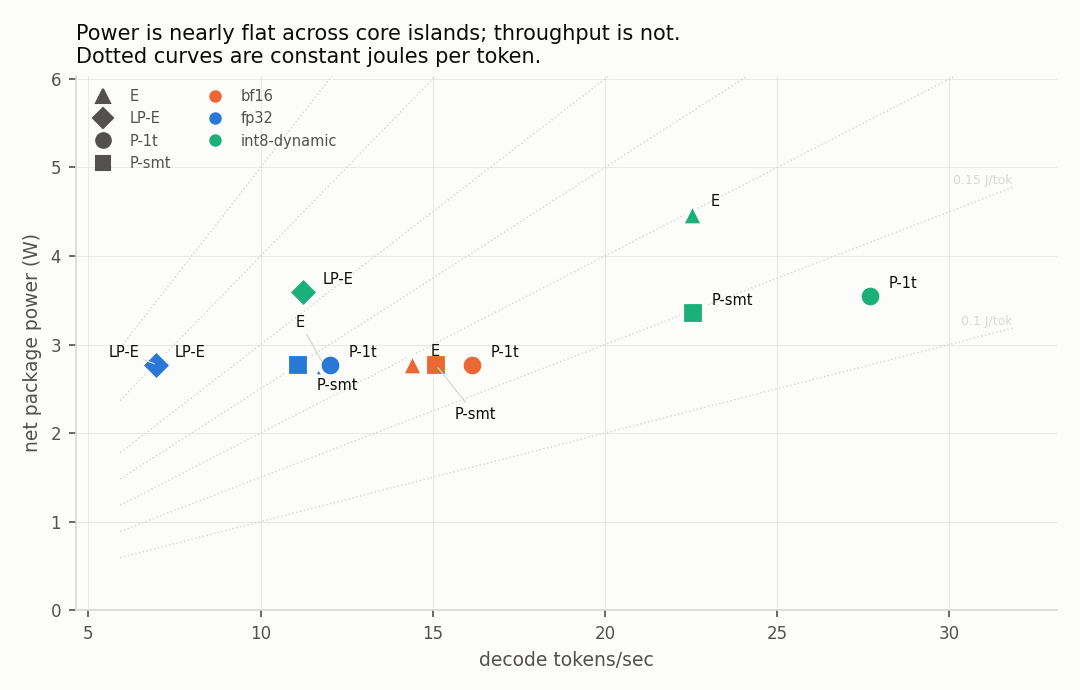
\includegraphics[width=0.78\textwidth]{figures/power_vs_throughput.png}
\caption{Net package power against decode throughput, one point per
configuration. fp32 (blue) and bf16 (orange) lie on a horizontal line at
2.77\,W while throughput varies more than twofold; only int8 (green) departs
from it. Dotted curves are constant joules per token, so a point's distance
along a curve is pure duration. This is the whole argument of
Section~\ref{sec:islands} in one panel.}
\label{fig:power}
\end{figure*}

With power constant, energy per token reduces to duration, and that is a
prediction rather than a description. Fig.~\ref{fig:power} shows the two
axes together, and Table~\ref{tab:identity} tests the prediction by
comparing each configuration's measured energy ratio against the inverse of its
independently measured throughput ratio.

\begin{table}[t]
\centering
\caption{Energy ratio against inverse throughput ratio, both measured. For the
memory-bound precisions the two agree within 1.1\%. int8, the one precision
whose power is not flat, is also the one where the identity fails.}
\label{tab:identity}
\begin{tabular}{llrrr}
\toprule
Precision & Placement & Energy & $1/$tput & Diff. \\
\midrule
fp32 & P-smt & 1.086 & 1.088 & $-0.16\%$ \\
fp32 & E     & 1.021 & 1.017 & $+0.42\%$ \\
fp32 & LP-E  & 1.737 & 1.727 & $+0.62\%$ \\
bf16 & P-smt & 1.073 & 1.069 & $+0.42\%$ \\
bf16 & E     & 1.148 & 1.136 & $+1.10\%$ \\
bf16 & LP-E  & 2.306 & 2.296 & $+0.43\%$ \\
\midrule
int8 & P-smt & 1.142 & 1.220 & $-6.39\%$ \\
int8 & E     & 1.558 & 1.222 & $\mathbf{+27.51\%}$ \\
int8 & LP-E  & 2.509 & 2.447 & $+2.54\%$ \\
\bottomrule
\end{tabular}
\end{table}

\begin{figure*}[t]
\centering
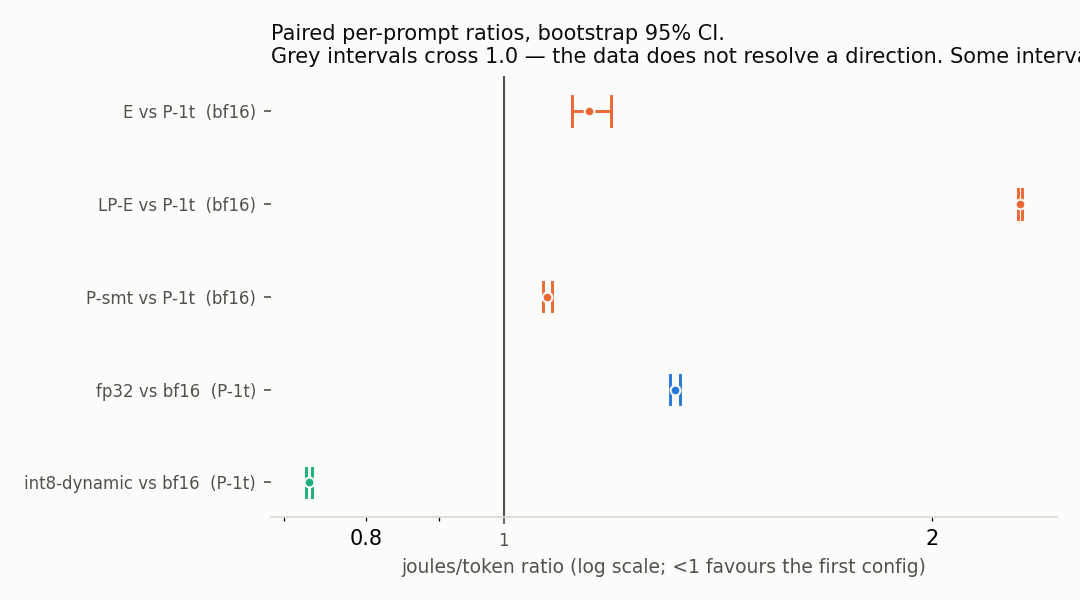
\includegraphics[width=0.78\textwidth]{figures/paired_ratios.png}
\caption{Paired per-prompt energy ratios with bootstrap 95\% intervals, log
scale, rule at unity. Every comparison in this study on one axis. Several
intervals are narrower than their marker.}
\label{fig:forest}
\end{figure*}

There is a name for what the power column shows. Barroso and
H\"{o}lzle~\cite{barroso2007proportional} argued that systems should be
\emph{energy-proportional}---that power should track utilisation---and observed
that real machines are not, drawing substantial power at low load. Our
measurement is that instance taken to its limit across a different axis: moving
the same work between islands changes utilisation of each island completely and
package power not at all. Where a system is perfectly non-proportional in this
sense, energy reduces to time, and the only available lever is to finish
sooner.

Two further consequences follow and are worth separating. The ordering is
robust: it rests on a $2.3\times$ duration difference against a power
difference of under 0.1\%, so no plausible baseline error inverts it. And the framing ``efficiency
cores save energy'' fails here not because the saving is small, but because
there is no power saving available to trade in the first place.

\subsection{The identity fails exactly where the mechanism predicts}
\label{sec:int8break}
int8 is the one precision whose power is not flat: it spans 13.96--15.92\,W,
median 14.81\,W. It is also the one precision for which the identity breaks,
by up to 27.5\% against a worst case of 1.10\% for fp32 and bf16
(Table~\ref{tab:identity}). Quantization moves work off the memory system and
back into the cores; power ceases to be flat, and duration ceases to be the
whole story.

We regard this as the strongest evidence for the explanation in
Section~\ref{sec:islands}. A flat-power observation alone is compatible with
several accounts. An account that also predicts \emph{where} flatness should
fail, and is then confirmed by the one precision that departs from it, is a
mechanism.

A second engine supports the same conclusion. Running GGUF models through
llama.cpp---a different runtime with its own kernels, written in C++ rather
than dispatched through PyTorch---reproduces the invariance: gross package
power is 14.01\,W for \texttt{Q4\_K\_M} and 13.99\,W for \texttt{Q8\_0},
spanning 16.4 to 31.7\,tok/s across the two islands, against the 14.00\,W
measured under PyTorch. The duration identity holds there too, to within 1.1\%
($1.660\times$ energy against $1.678$ inverse throughput for
\texttt{Q4\_K\_M}; $1.876$ against $1.884$ for \texttt{Q8\_0}). The flatness is
therefore a property of the platform under this workload rather than of one
inference framework.

The island penalty itself is smaller under llama.cpp ($1.66$--$1.88\times$
against $2.306\times$ for bf16 under PyTorch), which is expected: the ratio
depends on how completely an engine exploits the performance cores, and a
faster engine widens the gap it must then be penalised against. The direction
and the mechanism are unchanged; only the magnitude is engine-dependent, and we
report it as such.

\subsection{Precision, and its interaction with placement}
\label{sec:precision}
On the performance cores, fp32 costs $1.319\times$ [1.309, 1.330] the energy of
bf16 at $0.745\times$ the throughput, with perplexity marginally worse (12.449
against 12.427). bf16 is better on every axis measured.

That advantage is not uniform across islands:

\begin{center}
\begin{tabular}{lrr}
\toprule
Island & fp32/bf16 energy & fp32/bf16 tok/s \\
\midrule
P-1t  & 1.319 [1.309, 1.330] & 0.745 \\
P-smt & 1.335 [1.303, 1.367] & 0.732 \\
E     & 1.173 [1.132, 1.205] & 0.833 \\
LP-E  & \textbf{0.994 [0.989, 1.000]} & 0.991 \\
\bottomrule
\end{tabular}
\end{center}

\textbf{On the low-power island the bf16 advantage vanishes entirely.} fp32 and
bf16 reach the same 7.0\,tok/s and the same ${\approx}0.40$\,J/token. The
likely explanation is that the LP-E cores lack the bf16 instruction support
available on the performance cores, so bf16 executes at fp32 rates; confirming
this requires instruction-level profiling our harness does not perform, and we
record it as a hypothesis.

The consequence for scheduling is concrete: \textbf{precision and placement
cannot be chosen independently}. A runtime that migrates a bf16 workload to the
low-power island does not merely slow it by that island's ratio---it also
forfeits the entire benefit of the precision it was running.

\subsection{Per-tensor int8 saves energy and is still the wrong choice}
\label{sec:int8}
int8-dynamic on the performance cores costs $0.730\times$ [0.726, 0.733] the
energy per token of bf16: a 27\% saving, with the interval far from unity. The
saving is nonetheless unusable. Perplexity rises from 12.427 to 109.953, an
increase of 785\%, and needle retrieval falls from 3/3 to 0/3.

The result is therefore a cost--quality trade rather than an absence of
benefit. The question it raises is whether eight bits is simply too few, or
whether the fault lies in how the scale is assigned. We test this directly.

\subsection{Granularity, not bit width}
\label{sec:granularity}
Comparing a per-tensor 8-bit scheme against a per-block 4-bit scheme would vary
two things at once. We therefore add \texttt{Q8\_0}, a GGUF per-block scheme at
\emph{the same eight bits} as PyTorch's dynamic quantization, served through
llama.cpp. Bit width is then held constant and only granularity differs
(Table~\ref{tab:granularity}).

\begin{table}[t]
\centering
\caption{Quantization quality at matched bit width. \texttt{Q8\_0} and
int8-dynamic are both 8-bit and differ only in whether the scale is assigned
per block or per tensor. Perplexity over the same corpus and tokenizer in every
row.}
\label{tab:granularity}
\begin{tabular}{llrrr}
\toprule
Scheme & Engine & Bits & Granularity & $\Delta$ perplexity \\
\midrule
bf16         & PyTorch   & 16 & ---         & --- \\
\texttt{Q8\_0}   & llama.cpp & 8  & per-block   & $+4.7\%$ \\
int8-dynamic & PyTorch   & 8  & per-tensor  & $\mathbf{+785\%}$ \\
\texttt{Q4\_K\_M} & llama.cpp & 4  & per-block   & $+7.4\%$ \\
\bottomrule
\end{tabular}
\end{table}

At eight bits, per-block scaling costs 4.7\% perplexity and per-tensor scaling
costs 785\%: a factor of 167 in quality damage attributable to granularity
alone, with bit width fixed. Halving the bit width to four, while keeping
per-block scales, costs 7.4\%---still two orders of magnitude less than the
8-bit per-tensor scheme. Bit width is not the operative variable on this
workload; granularity is. The finding is consistent with the quantization
literature~\cite{dettmers2022llmint8,frantar2023gptq,lin2024awq,
xiao2023smoothquant,gholami2022quantsurvey}, and we contribute the energy
accounting rather than the scheme.

Two caveats bound what this comparison supports. The per-block schemes are
served by a different runtime, so any \emph{energy} difference between engines
confounds quantization with implementation and we do not report one as a
finding; the perplexity comparison is unaffected, since every row is scored
over the same corpus with the same tokenizer. And a quality probe this thin
(Section~\ref{sec:method}) establishes that a scheme has not collapsed, not
that it is equivalent to full precision.

\subsection{Quantization does not shrink the KV cache}
Dynamic quantization touches only Linear weights, so the KV cache remains at
the unquantized dtype. The measured per-step curves for fp32 and int8 are
byte-identical, both reaching 6{,}408\,KiB after 256 decode steps, while bf16
reaches exactly half at 3{,}204\,KiB (Fig.~\ref{fig:kv}). For long-context work, where
the cache rather than the weights dominates footprint, per-tensor int8
therefore offers no relief on the axis that matters while bf16 offers a factor
of two.

\begin{figure}[t]
\centering
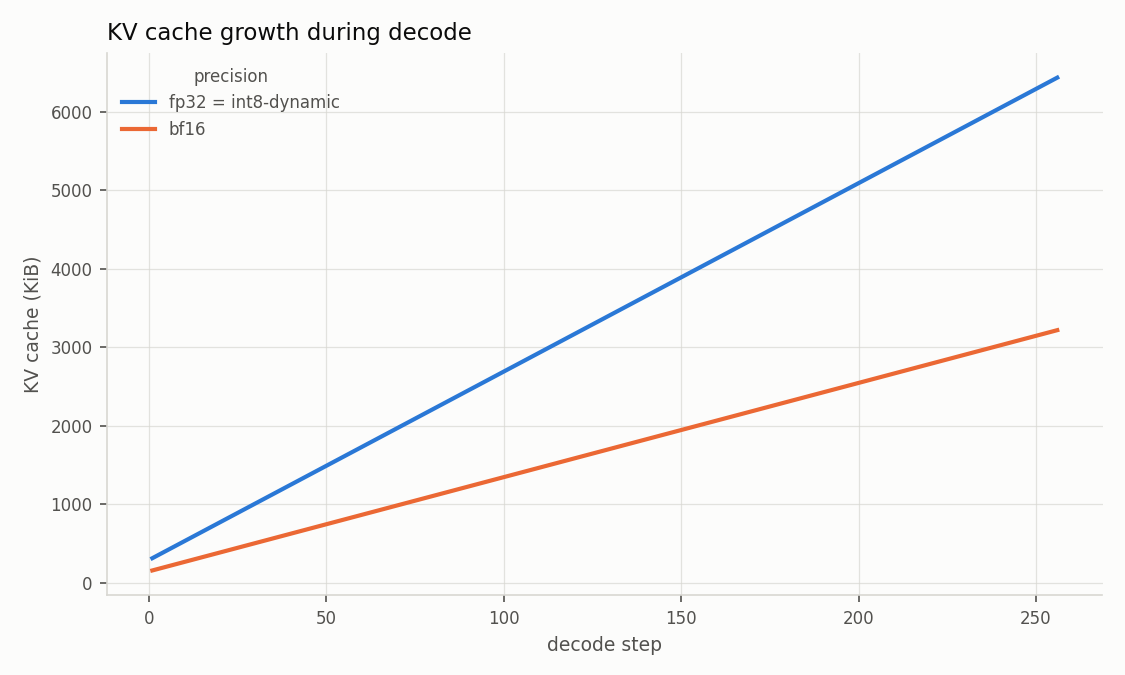
\includegraphics[width=\columnwidth]{figures/kv_growth.png}
\caption{KV cache size at every decode step. fp32 and int8-dynamic are
byte-identical because dynamic quantization touches only Linear weights; bf16
is exactly half. Quantizing weights does not help on the axis that dominates
long-context footprint.}
\label{fig:kv}
\end{figure}

\subsection{Placement changes the arithmetic, not the output}
\label{sec:determinism}
Greedy decode produced byte-identical generated text on all four islands, for
every precision and prompt, verified by digest. Placement affects cost, not
tokens.

The arithmetic beneath is not identical. int8 perplexity varies by placement
across a 4\% range---106.391 on LP-E against 110.608 on E---while fp32 and bf16
perplexity is constant to three decimal places. Different islands dispatch
quantized kernels differently and the numerics differ measurably; greedy argmax
is simply robust to a difference of that size.

Three consequences, in increasing order of practical weight. Any claim of
bit-exact reproducibility across islands is false for quantized models, which
matters for regression testing and for auditing a deployed system. A
sampling-based decoder has no argmax margin to absorb the difference, so the
invariance observed here does not transfer to it. And a scheduler that migrates
a quantized workload between islands mid-generation is changing the arithmetic
underneath a partially-built KV cache: our measurements cannot say whether that
is harmless, because we never migrate mid-generation, and we flag it as a
hazard that heterogeneous-aware runtimes should establish before relying on
free migration.

\subsection{Prefill behaves oppositely, and confirms the mechanism}
\label{sec:prefill}
The argument of this paper rests on decode being memory-bound while prefill is
not (Section~\ref{sec:phases}). Because the harness times the two phases
separately, that premise can be tested rather than assumed, on the same
hardware in the same runs.

Simultaneous multithreading provides the test. Its effect reverses between the
phases (Table~\ref{tab:prefill}): enabling SMT makes prefill $1.193\times$
faster and decode $0.936\times$ slower, with both intervals excluding unity.
This is precisely the signature the two-regime account predicts. A
compute-bound phase leaves issue slots idle that a sibling thread can fill, so
SMT helps; a memory-bound phase is already waiting on DRAM, so the sibling adds
cache contention and no useful parallelism.

\begin{table}[t]
\centering
\caption{Throughput ratios against P-1t, bf16, paired per-prompt. SMT helps the
compute-bound phase and hurts the memory-bound one; the low-power island is
relatively worse at prefill, which is the compute-bound phase.}
\label{tab:prefill}
\begin{tabular}{lrr}
\toprule
Placement & Prefill & Decode \\
\midrule
P-smt & \textbf{1.193 [1.102, 1.370]} & \textbf{0.936 [0.926, 0.943]} \\
E     & 0.933 [0.809, 1.012] & 0.881 [0.860, 0.901] \\
LP-E  & 0.370 [0.367, 0.374] & 0.435 [0.434, 0.437] \\
\bottomrule
\end{tabular}
\end{table}

The low-power island shows the same asymmetry from the other direction. It
reaches $0.435\times$ the performance island's decode throughput but only
$0.370\times$ its prefill throughput: relatively worse at the phase that
demands compute. The E-core prefill ratio is the one comparison in this table
whose interval spans unity, and we draw no conclusion from it.

Prefill nonetheless contributes little to the energy totals reported here,
accounting for 2.3\% of the measurement window on P-1t and 2.7\% on LP-E at 256
generated tokens. That is why the rest of this paper reports decode: at
realistic generation lengths it is almost the entire cost. The phases are
separated so that this could be established rather than assumed, and so that
the premise underlying the mechanism could be tested independently.

\subsection{Generalisation: model scale and context length}
\label{sec:generalisation}
Two further experiments bound the result. Both use the protocol of
Section~\ref{sec:method} without modification.

\paragraph{Model scale} Repeating the full matrix on SmolLM2-135M, a model
roughly a quarter the size, does not weaken the effect---it strengthens it
(Table~\ref{tab:scale}). The penalty for placing decode on the low-power island
is 61\% larger on the smaller model, and the duration identity holds on both.

\begin{table}[t]
\centering
\caption{The island penalty against model size, bf16, paired per-prompt.
The identity of Section~\ref{sec:islands} holds on both models.}
\label{tab:scale}
\begin{tabular}{lrr}
\toprule
Model & LP-E vs.\ P-1t energy & Identity error \\
\midrule
Qwen2.5-0.5B & 2.306 [2.301, 2.314] & $+0.43\%$ \\
SmolLM2-135M & \textbf{3.712 [3.159, 4.342]} & $+0.68\%$ \\
\bottomrule
\end{tabular}
\end{table}

The mechanism is visible in the throughput. The performance cores exploit the
smaller model---16.1 to 34.7\,tok/s, a $2.2\times$ gain---while the low-power
island barely moves, 7.0 to 8.3\,tok/s, a $1.2\times$ gain. Less weight traffic
makes the workload relatively less memory-bound, so core capability begins to
matter, and that is precisely what the low-power island does not supply.

The same mechanism erases the quantization benefit. On SmolLM2, int8 costs
$1.053\times$ [1.007, 1.101] the energy of bf16---marginally \emph{more}
expensive, with the interval excluding unity on the opposite side to the
$0.730\times$ measured on Qwen. Quantization saves energy only to the degree the
model is memory-bound; perplexity still rises from 13.4 to 40.8. We note that
the needle probe carries no signal at this model size, SmolLM2-135M being a base
model rather than instruction-tuned, and do not report it as a quality
comparison there.

Package power was again flat: medians of 14.00\,W for fp32 and bf16 and
14.26\,W for int8, on a different model and against a different idle baseline
(9.66\,W). This is the third independent observation of the invariance.

\paragraph{Context length} Generating 1024 tokens rather than 256 quadruples the
KV cache, from 3{,}204 to 12{,}384\,KiB, and costs both islands about 12\%
throughput as attention over a longer context grows more expensive. The ratio is
essentially unmoved: $2.251\times$ against $2.306\times$, with package power
still exactly 14.00\,W on both islands at four times the context length.

We report this comparison without an interval. It was run with two prompts
rather than four, leaving two paired ratios---below the three our bootstrap
procedure requires before it will report one (Section~\ref{sec:stats}). The
point estimate is sound and the conclusion is stable across the two lengths, but
we flag the limitation rather than present a number the design cannot support.

\subsection{The Pareto frontier is necessary, not sufficient}
The frontier contains \texttt{bf16/P-1t}, \texttt{int8/P-1t} and
\texttt{int8/P-smt}. Two of the three score 0/3 on needle retrieval and carry a
785\% perplexity penalty (Fig.~\ref{fig:pareto}): non-dominated because
genuinely cheaper, and genuinely unusable.

\begin{figure}[t]
\centering
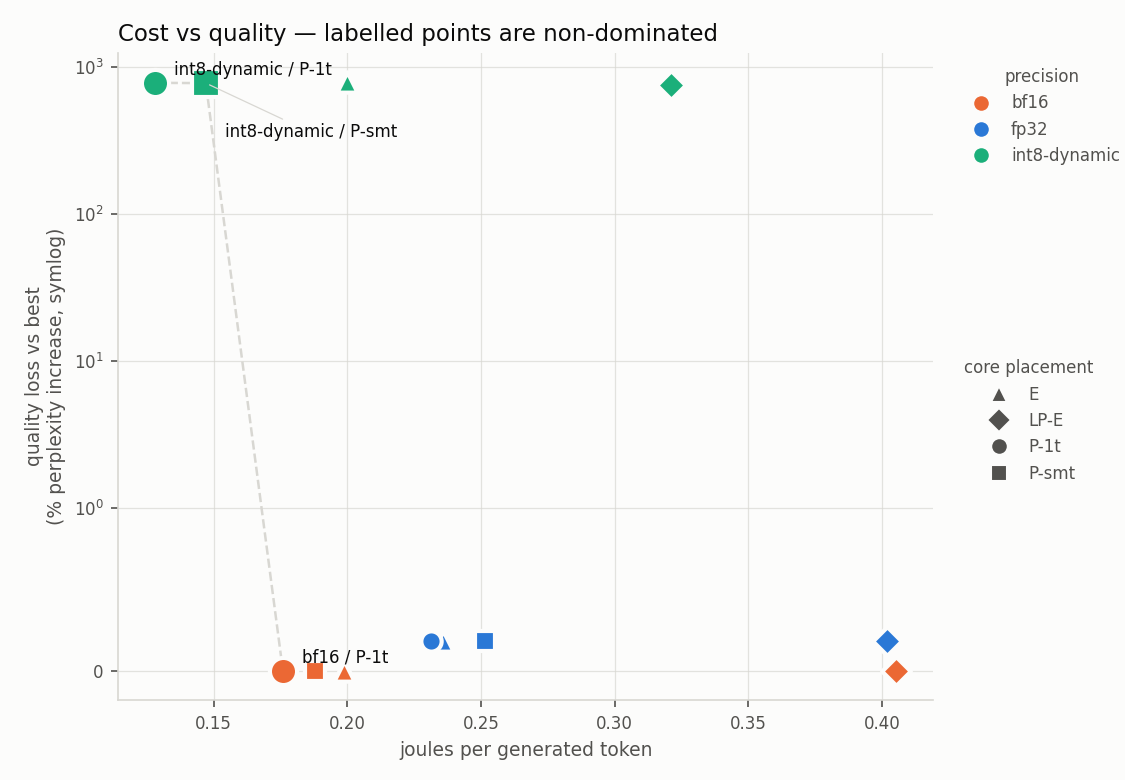
\includegraphics[width=\columnwidth]{figures/pareto.png}
\caption{Cost against quality loss, frontier dashed. Two of the three
non-dominated configurations are int8 variants that score 0/3 on needle
retrieval: cheaper, and unusable.}
\label{fig:pareto}
\end{figure}

This is a limitation of the method rather than a result. A frontier identifies
what is not dominated, not what is worth choosing, and must be read alongside
the quality column rather than instead of it. The actionable output of this
study is bf16 on the performance cores, one thread per core.

% ---------------------------------------------------------------------------
\section{Discussion}

\subsection{Implications for schedulers}
The practical recommendation is the opposite of the one the island naming
suggests: on this class of part, sustained LLM decode should not be migrated to
the efficiency or low-power islands in pursuit of energy savings. Doing so
costs $1.148\times$ and $2.306\times$ the energy per token respectively, and
returns nothing, because there is no power reduction to collect.

The generalisable form of the recommendation is not ``use the big cores''. It
is that the question is settled by one measurement: whether package power
varies across islands for the workload in question. Where it does, a
power--duration trade exists and migration can win. Where it does not---as here,
because decode is memory-bound---migration only buys duration, and duration is
the entire cost.

A second consequence is that a runtime cannot treat precision and placement as
independent knobs. Migrating a bf16 workload to the low-power island forfeits
the bf16 advantage entirely (Section~\ref{sec:precision}), so the cost of
migration is larger than the island ratio alone implies.

\subsection{Implications for practitioners}
For deployment on this class of hardware: bf16 on the performance cores, one
thread per core. SMT costs throughput at every precision and on both models
measured---6--18\% on Qwen2.5-0.5B and 16--23\% on SmolLM2-135M---which is the
expected behaviour for a memory-bound workload whose sibling thread adds
contention without adding useful parallelism.

Throughput should not be used as a proxy for energy without first checking that
power is flat. Where it is flat the proxy is exact, and where it is not---int8
here---it misleads by up to 27\%.

Finally, quantization should be evaluated at the level of scale granularity
rather than bit width. The scheme measured here is fast, genuinely cheaper in
energy, and unusable.

\subsection{What the difference is worth}
\label{sec:sustainability}
Work on the sustainability of machine learning has concentrated on
training~\cite{strubell2019energy,patterson2021carbon}, on reporting
standards~\cite{henderson2020reporting}, and on the argument that efficiency
should count alongside accuracy as a research
objective~\cite{schwartz2020greenai}. Inference at the edge has received less
attention, and the quantity this paper measures is small per event and large
only in aggregate, which is the characteristic shape of an efficiency result
worth acting on. It is worth stating the magnitude explicitly rather than leaving the
reader to assume it.

The avoidable energy is the gap between the best and worst placement at fixed
precision and byte-identical output: $0.4053 - 0.1758 = 0.2295$\,J per
generated token (Table~\ref{tab:main}). A device generating
$10^{4}$ tokens per day---on the order of twenty to thirty short interactions,
and the weakest assumption in what follows---therefore wastes 838\,kJ, or
0.233\,kWh, over a year by scheduling decode on the low-power island. At the
2025 global average grid intensity of 458\,gCO\textsubscript{2}e/kWh~\cite{ember2026review}
that is 107\,gCO\textsubscript{2}e per device per year; the IEA's
CO\textsubscript{2}-only figure of 435\,g/kWh~\cite{iea2026electricity} gives
101\,g.

Across a population the arithmetic is linear. Gartner places 2025 AI-PC
shipments at 77.8 million units~\cite{gartner2025aipc}. One cohort of that size,
under the same assumption, accounts for \textbf{18.1\,GWh and roughly
8\,300 tonnes CO\textsubscript{2}e per year} attributable to a single
scheduling decision. Table~\ref{tab:scale} gives the sensitivity to the token
rate, which dominates the estimate.

\begin{table}[t]
\centering
\caption{Avoidable energy from placement, scaled. The $2.306\times$ ratio is
measured; everything else is arithmetic over stated assumptions. The estimate
is linear in the token rate, which is the least certain input.}
\label{tab:scale}
\begin{tabular}{rrrr}
\toprule
Tokens/device/day & kWh/device/yr & GWh/yr & tCO\textsubscript{2}e/yr \\
\midrule
1\,000  & 0.023 & 1.8  & 830 \\
5\,000  & 0.116 & 9.1  & 4\,150 \\
10\,000 & 0.233 & 18.1 & 8\,290 \\
50\,000 & 1.163 & 90.5 & 41\,460 \\
\bottomrule
\end{tabular}
\end{table}

Three qualifications keep this honest. The figures assume every device makes
the worse choice, so they bound the opportunity rather than describe current
waste. They cover only the cohort shipped in a single year, and say nothing
about the installed base. And they are linear in a token rate we have not
measured and that no public figure establishes well.

What makes the quantity interesting is not its size but its cost. It requires
no new hardware, no accuracy sacrifice and no change to the model: the output
is byte-identical across placements (Section~\ref{sec:determinism}). It is
recovered by scheduling, which is among the cheapest interventions available in
a field whose efficiency gains usually demand retraining, quantization or
silicon. Against the energy of training the models being served it is
negligible; against the cost of obtaining it, it is nearly free.

\section{Threats to Validity}
\label{sec:threats}
\emph{One machine, one SoC generation.} Nothing here generalises beyond Meteor
Lake without further measurement. The result is explicitly a property of a
platform whose package power is flat across islands for this workload; a part
on which that does not hold would behave differently, and
Section~\ref{sec:contradiction} discusses one that apparently does not.

\emph{Model scale.} Models below 1\,B parameters, bounded by available memory.
Section~\ref{sec:generalisation} shows the ordering holds across a $4\times$
range of model size and that the penalty grows as models shrink, but 7\,B---%
where memory pressure is far higher and package power may cease to be flat---%
remains untested and is the most likely place these conclusions break.

\emph{Idle baseline.} Net energy is gross minus idle power times duration, and
the baseline is the least trustworthy term in that expression. Here it is
11.23\,W against a gross draw of 14.00\,W, so it accounts for roughly 80\% of
each reading and the net signal is the remaining 2.77\,W. This is the strongest
argument for reporting ratios rather than absolute joules: if two
configurations draw equal power, their net energy ratio equals their duration
ratio whatever baseline is subtracted, so every comparison in
Section~\ref{sec:results} is baseline-independent while the absolute figures in
Table~\ref{tab:main} are not. An earlier iteration of this study measured
24-token generations, where the baseline exceeded the net signal outright; we
report that dataset and its failures alongside this one. We also report a
failed attempt at a per-configuration baseline which made the data substantially
noisier, and the reason: a baseline sampled immediately after a burst of work
captures the CPU decaying out of turbo rather than idling.

\emph{Batch size one.} Every measurement is unbatched. Batching amortises each
weight read across several sequences, raising arithmetic intensity and moving
decode back toward the compute-bound regime, so the power invariance reported
here should not be assumed to survive it. The single-request case is the
on-device regime this paper addresses; batched serving is a different setting
and an obvious next measurement.

\emph{Package domain includes the iGPU.} CPU and iGPU energy cannot be fully
separated within a run on an integrated part.

\emph{No external instrument.} We did not validate RAPL against a wall meter or
a shunt on this part. We rely on published characterisation of RAPL against
full-system power~\cite{khan2018rapl} rather than on a measurement of our own,
which is a dependency worth naming. It bears mainly on absolute joules; the
comparisons in Section~\ref{sec:results} are ratios taken from the same counter
under identical conditions, where a systematic instrument offset cancels.

\emph{Quality measure.} Perplexity and a single needle probe are thin, and the
needle probe carries no signal on a base model: SmolLM2-135M fails it at every
precision, so it cannot discriminate there and we do not use it to. It was
adequate for its purpose, which was detecting the int8 collapse on the
instruction-tuned model, and nothing more.

\emph{No hardware performance counters.} The SMT penalty and the bf16/LP-E
equivalence are both inferred from throughput. Cache-miss and stall-cycle
counters would convert both from plausible accounts into measurements, and the
missing-bf16-support explanation in Section~\ref{sec:precision} in particular
remains a hypothesis.

\emph{Machine quiescence.} The host was a laptop in ordinary use and some
trials show excursions consistent with background load. This widens intervals
rather than biasing them in a particular direction, so the effects reported
here are if anything understated.

% ---------------------------------------------------------------------------
\section{Related Work}

\subsection{A contradicting result on ARM mobile, and why both can hold}
\label{sec:contradiction}
The conclusion reached here is the opposite of the one reached by
MNN-AECS~\cite{mnn2025aecs}, which reduces LLM decoding energy on mobile
devices precisely by \emph{dynamically selecting low-power CPU cores}, reporting
a 23\% energy reduction across five Android and two iOS devices. Our measurement
says that placing decode on the low-power island costs $2.306\times$ the
energy per token. The disagreement is not incidental and we do not attempt to
explain it away; it is the most important thing to settle about this result.

We believe both findings are correct on their own platforms, and that the
difference is a property of the hardware rather than of the methodology. Three
distinctions matter.

\emph{The islands are not analogous.} ARM big.LITTLE pairs out-of-order
performance cores with genuinely low-power in-order cores designed to run at a
small fraction of the big cores' power. Intel's E-cores are throughput-oriented
rather than low-power-oriented: they exist to deliver area-efficient
multithreaded throughput, not to sip power. Only the LP-E island is positioned
as a low-power domain, and it contains two cores. The name ``efficiency core''
spans two quite different design intents across the two ecosystems.

\emph{The power floor differs.} Our central measurement is that net package
power is approximately invariant across islands (Section~\ref{sec:islands}). On
a part where the low-power island does achieve a substantially lower operating
power, the trade that MNN-AECS exploits is available and ours is not. The
question is empirical for each platform, and the answer we report is specific
to the one we measured.

\emph{The objective differs.} MNN-AECS optimises energy subject to an accepted
slowdown threshold. Where power is flat, no such trade exists: slowing down
costs energy proportionally and buys nothing.

The contribution of this paper is therefore narrower and, we think, more useful
than ``efficiency cores do not save energy''. It is that the mobile result does
not transfer to x86 heterogeneous SoCs, that the reason is measurable rather
than conjectural, and that the measurement needed to tell the two cases apart
is a single one: whether package power varies across islands for the workload
in question.

\subsection{Energy of LLM inference}
Most published energy figures for LLM inference describe datacenter GPUs.
Samsi et al.~\cite{samsi2023words} benchmark multi-node, multi-GPU inference at
scale, and Luccioni et al.~\cite{luccioni2024power} compare the deployment cost
of model categories in energy and carbon per thousand inferences, establishing
that generative architectures are orders of magnitude more expensive than
task-specific ones. Both measure at the scale and on the hardware where most
inference tokens are currently produced.

Characterisation at the edge is more recent and more fragmented. Zhang and
Huang~\cite{cpuoutperform2025} report cases in which CPUs outperform integrated
GPUs for on-device inference. Taherin et al.~\cite{hydra2026} characterise
inference across edge SoC generations, backends and quantization levels, and
Zhang et al.~\cite{mobiledvfs2025} show that independently operating CPU, GPU
and memory frequency governors leave substantial latency on the table at equal
energy. What this body of work does not yet provide, and what we contribute, is
a ground-truth energy comparison across the \emph{core islands of a single x86
SoC} at fixed output, with the power and duration terms reported separately
rather than multiplied together.

\subsection{Why decode is memory-bound}
The separation of prefill and decode into a compute-bound and a memory-bound
phase is established by roofline analysis of transformer
inference~\cite{yuan2024roofline}: prefill reuses weights across the whole
prompt and sits near or beyond the ridge point, while single-token decode is a
sequence of matrix--vector products at roughly one FLOP per byte. Serving
systems are built around the consequence, managing memory rather than
arithmetic as the scarce resource~\cite{kwon2023pagedattention}, and the
major inference optimisations attack the same bottleneck from different
directions: restructuring attention to reduce memory
traffic~\cite{dao2022flashattention}, or amortising the per-token weight read
across several candidate tokens~\cite{leviathan2023speculative}. All three
presuppose that decode is memory-bound; we measure a consequence of that
premise rather than assuming it.

We rely on this property for the mechanism in Section~\ref{sec:islands}: if the
bottleneck is off-core, the identity of the cores issuing the loads has little
influence on the power drawn, and the energy a placement costs is set by how
long it occupies the memory system. To our knowledge this consequence has not
previously been measured directly as package power invariance across
heterogeneous islands.

\subsection{Race to idle}
Whether to run fast and sleep or to run slowly and stay busy is a long-settled
question in the abstract and a workload-dependent one in practice. Le Sueur and
Heiser~\cite{lesueur2011slowdown} examine the decline of DVFS effectiveness as
static power grows and idle states improve; Albers and
Antoniadis~\cite{albers2014race} give the theoretical treatment of speed
scaling with a sleep state; Awan and Petters~\cite{awan2014racetohalt} develop
race-to-halt strategies for embedded real-time systems; and Kim et
al.~\cite{kim2015racing} analyse racing and pacing heuristics both
theoretically and empirically, finding that neither dominates universally.

The usual framing of this debate presupposes a power--frequency trade: running
slower is assumed to draw less power, and the question is whether the saving
offsets the longer runtime. Our contribution to this line is a workload for
which the premise fails outright. Across islands, running slower draws
\emph{the same} power (Section~\ref{sec:islands}), so there is no trade to
evaluate and racing wins by default. We regard this as a sharper case than the
ones usually studied rather than a new heuristic.

\subsection{Heterogeneous and asymmetric multicore energy}
The intuition that migrating work to smaller cores saves energy was developed
on ARM big.LITTLE and related asymmetric designs. Catal\'{a}n et
al.~\cite{catalan2015bigLITTLE} optimise matrix multiplication across
asymmetric cores for performance and energy jointly; Butko et
al.~\cite{butko2019exploration} explore the trade-off space across
heterogeneous configurations; and Coutinho et al.~\cite{coutinho2020tradeoffs}
measure performance and energy for parallel applications on heterogeneous
multi-processing systems. This literature establishes both that the trade is
real on those parts and that it is workload-dependent.

Two things make the present setting different. The workload is sustained and
memory-bound rather than bursty and compute-bound, which is the regime in which
the premise of the trade is most likely to fail. And the hardware divides
differently: Intel's E-cores are throughput-oriented rather than
low-power-oriented (Section~\ref{sec:background}), so a result established on
big.LITTLE does not transfer on the strength of the shared label alone.
Section~\ref{sec:contradiction} works through the one case where this matters
most.

\subsection{Quantization granularity}
Post-training quantization of LLM weights is a mature area, and its consistent
lesson is that the assignment of scales matters at least as much as the
remaining bit width. LLM.int8()~\cite{dettmers2022llmint8} isolates outlier
features for higher-precision treatment; GPTQ~\cite{frantar2023gptq} performs
second-order-informed per-layer rounding; AWQ~\cite{lin2024awq} scales channels
by activation magnitude and targets on-device deployment specifically;
SmoothQuant~\cite{xiao2023smoothquant} migrates activation outliers into the
weights so that both can be quantized. All preserve quality at bit widths where
uniform per-tensor schemes fail, and the broader
survey~\cite{gholami2022quantsurvey} frames granularity as a primary design
axis rather than an implementation detail.

The scheme we measure sits at the naive end of that spectrum deliberately. Our
contribution here is not a new quantization method but an energy accounting of
one: we show that the per-tensor scheme is genuinely cheaper in energy, by
27\%, and that the quality cost makes the saving unusable---so the relevant
design axis for energy-aware deployment is granularity, not bit width.

\subsection{RAPL as an instrument}
Khan et al.~\cite{khan2018rapl} characterise RAPL against full-system power on
production hardware, reporting close agreement, negligible overhead and
microsecond-scale counter updates. The counters' unprivileged accessibility was
subsequently removed: PLATYPUS~\cite{lipp2021platypus} recovers AES-NI keys
from SGX enclaves and defeats KASLR through RAPL alone, and related work
extracts further secrets through RAPL-induced side
channels~\cite{zhang2021redalert}. Any reproduction of measurements like ours
therefore requires a deliberate relaxation of permissions, which we document in
the artifact rather than leave implicit.

\section{Conclusion}
On a heterogeneous consumer SoC, the island named for efficiency is not the
efficient choice for LLM decode. The low-power island costs $2.306\times$ the
energy per generated token of the performance island, and it does so for a
reason that is measurable rather than conjectural: package power is flat at
14.00\,W across islands, so energy per token is duration, and a slower island
is simply a more expensive one. The measured energy ratios match inverse
throughput to within 1.1\% wherever power is flat, and depart from it---by up
to 27.5\%---for the one precision where power is not.

The underlying cause is that decode is memory-bandwidth-bound, which makes the
result portable as a method even where it is not portable as a number. A
platform whose low-power island does achieve materially lower power under this
workload would admit the trade our platform denies, and such a result has been
reported on ARM mobile. The two findings are reconciled by a single
measurement, which we recommend as the first thing to check before scheduling
inference across heterogeneous cores: does package power vary across islands
for this workload? If it does not, there is nothing to trade, and the right
policy is to race to idle.

\section*{Acknowledgment}
The author used Anthropic's Claude (Claude Opus 5) as a writing and engineering
assistant. It contributed to drafting the manuscript text, to the statistical
analysis code---paired per-prompt ratios, bootstrap confidence intervals---and
figure generation in \texttt{analyze.py}, and to corrections of the measurement
harness. The research questions, experimental design, all measurements, and the
interpretation of results are the author's own. The author takes full
responsibility for the content.

\section*{Artifact Availability}
The measurement harness, the complete dataset including every discarded run,
and the analysis that generates every table and figure in this paper are
archived under a permanent DOI\ifanon, withheld for double-anonymized review
because the repository identifies the author and supplied on the title page\else{} at
\href{https://doi.org/10.5281/zenodo.23243516}{doi:10.5281/zenodo.23243516}\fi.
Five superseded runs are included
deliberately, each with a written account of why it was rejected---short
measurement windows, prompts cycled by repeat index, an unsettled warmup, a
per-configuration baseline that made the data noisier, and a half-measured
dataset---because the reason a measurement was discarded is part of the method.

\bibliographystyle{IEEEtran}
\bibliography{refs}

\ifanon
% Biography omitted for double-anonymized review.
\else
% IEEEbiographynophoto avoids needing a portrait at submission. Switch to
% \begin{IEEEbiography}[{\includegraphics[...]{photo}}]{...} if a photo is
% wanted for the camera-ready version.
\begin{IEEEbiographynophoto}{Muhammad Etisam Ul Haq}
received the B.S. degree in data science from the Punjab University College of
Information Technology (PUCIT), University of the Punjab, Lahore, Pakistan, and
is currently pursuing the M.S. degree in data science at the Institute of Data
Science, University of Engineering and Technology, Lahore, Pakistan.

He works as a machine learning engineer, where his practice covers large
language model fine-tuning and inference serving, retrieval-augmented
generation, and private inference on non-CUDA accelerators. His research
interests include the energy efficiency of on-device machine learning,
measurement methodology for heterogeneous processors, and the systems side of
language model deployment.
\end{IEEEbiographynophoto}
\fi

\end{document}
